% ------------------------------------------------------------------------
% ------------------------------------------------------------------------
% abnTeX2: Modelo de Trabalho Academico (tese de doutorado, dissertacao de
% mestrado e trabalhos monograficos em geral) em conformidade com 
% ABNT NBR 14724:2011: Informacao e documentacao - Trabalhos academicos -
% Apresentacao
% ------------------------------------------------------------------------
% ------------------------------------------------------------------------
\documentclass[
	% -- opções da classe memoir --
	12pt,						% tamanho da fonte
	openright,					% capítulos começam em pág ímpar (insere página vazia caso preciso)
	twoside,					% para impressão em verso e anverso. Oposto a oneside
	a4paper,					% tamanho do papel. 
				% -- opções da classe abntex2 --
	%chapter=TITLE,			% títulos de capítulos convertidos em letras maiúsculas
	%section=TITLE,			% títulos de seções convertidos em letras maiúsculas
	%subsection=TITLE,			% títulos de subseções convertidos em letras maiúsculas
	%subsubsection=TITLE,		% títulos de subsubseções convertidos em letras maiúsculas
				% -- opções do pacote babel --
	english,					% idioma adicional para hifenização
	spanish,					% idioma adicional para hifenização
	brazil					% o último idioma é o principal do documento
	]{abntex2}

\usepackage{mystyle}

% ---
% Informações de dados para CAPA e FOLHA DE ROSTO
% ---
\titulo{Avaliação das Condições de Segurança do Trabalho e Saúde Ocupacional em um Navio de Contenção de Óleo}
\autor{Henrique Mageste}
\local{Rio de Janeiro, RJ - Brasil}
\data{\today}
\orientador{Justino Sanson Wanderley da Nóbrega, M. Sc.}
%\coorientador{Equipe \abnTeX}
\instituicao{%
  Universidade Federal do Rio de Janeiro - UFRJ
  \par
  Engenharia de Segurança do Trabalho
  \par
  Programa de Pós-Graduação}
\tipotrabalho{Monografia}
\preambulo{Monografia Submetida ao Corpo Docente do Curso de Pós-Graduação em Engenharia de Segurança do Trabalho
da Universidade Federal do Rio de Janeiro como Parte dos Requisitos Necessários para Obtenção do Título de Especialista
em Engenharia de Segurança do Trabalho}
% ---

\makeindex

\begin{document}
\selectlanguage{brazil}
\frenchspacing					% Retira espaço extra obsoleto entre as frases

% ----------------------------------------------------------
% ELEMENTOS PRÉ-TEXTUAIS
% ----------------------------------------------------------
%\pretextual

\imprimircapa
\imprimirfolhaderosto*		% o * indica que haverá a ficha bibliográfica

% Isto é um exemplo de Ficha Catalográfica, ou ``Dados internacionais de
% catalogação-na-publicação''. Você pode utilizar este modelo como referência. 
% Porém, provavelmente a biblioteca da sua universidade lhe fornecerá um PDF
% com a ficha catalográfica definitiva após a defesa do trabalho. Quando estiver
% com o documento, salve-o como PDF no diretório do seu projeto e substitua todo
% o conteúdo de implementação deste arquivo pelo comando abaixo:
%
% \begin{fichacatalografica}
%     \includepdf{fig_ficha_catalografica.pdf}
% \end{fichacatalografica}

\begin{fichacatalografica}
	\sffamily
	\vspace*{\fill}					% Posição vertical
	\begin{center}					% Minipage Centralizado
	\fbox{\begin{minipage}[c][8cm]{13.5cm}		% Largura
	\small
	\imprimirautor
	%Sobrenome, Nome do autor
	
	\hspace{0.5cm} \imprimirtitulo  / \imprimirautor. --
	\imprimirlocal, \imprimirdata-
	
	\hspace{0.5cm} \pageref{LastPage} p. : il. (algumas color.) ; 30 cm.\\
	
	\hspace{0.5cm} \imprimirorientadorRotulo~\imprimirorientador\\
	
	\hspace{0.5cm}
	\parbox[t]{\textwidth}{\imprimirtipotrabalho~--~\imprimirinstituicao,
	\imprimirdata.}\\
	
	\hspace{0.5cm}
		1. Palavra-chave1.
		2. Palavra-chave2.
		2. Palavra-chave3.
		I. Orientador.
		II. Universidade xxx.
		III. Faculdade de xxx.
		IV. Título 			
	\end{minipage}}
	\end{center}
\end{fichacatalografica}
% Isto é um exemplo de Folha de aprovação, elemento obrigatório da NBR
% 14724/2011 (seção 4.2.1.3). Você pode utilizar este modelo até a aprovação
% do trabalho. Após isso, substitua todo o conteúdo deste arquivo por uma
% imagem da página assinada pela banca com o comando abaixo:
%
% \includepdf{folhadeaprovacao_final.pdf}
%
\begin{folhadeaprovacao}

  \begin{center}
    {\ABNTEXchapterfont\large\imprimirautor}

    \vspace*{\fill}\vspace*{\fill}
    \begin{center}
      \ABNTEXchapterfont\bfseries\Large\imprimirtitulo
    \end{center}
    \vspace*{\fill}
    
    \hspace{.45\textwidth}
    \begin{minipage}{.5\textwidth}
        \imprimirpreambulo
    \end{minipage}%
    \vspace*{\fill}
   \end{center}
        
   Trabalho aprovado. \imprimirlocal, \today:

   \assinatura{\textbf{\imprimirorientador} \\ Orientador} 
   \assinatura{\textbf{Professor} \\ Convidado 1}
   \assinatura{\textbf{Professor} \\ Convidado 2}
      
   \begin{center}
    \vspace*{0.5cm}
    {\large\imprimirlocal}
    \par
    {\large\imprimirdata}
    \vspace*{1cm}
  \end{center}
  
\end{folhadeaprovacao}
\begin{dedicatoria}
   \vspace*{\fill}
   \centering
   \noindent
   \textit{Este trabalho é dedicado a todos os engenheiros,\\
	   de segurança ou não, que queiram se aventurar na\\
	   legislação naval.} \vspace*{\fill}
\end{dedicatoria}
\begin{agradecimentos}
Os agradecimentos principais são direcionados ao professor Justino da Nóbrega,
pela sua paciência e orientação durante todo o curso deste trabalho.

Agradecimentos especiais são direcionados à empresa e à sua coordenadora ambiental que
possibilitaram o desenvolvimento deste trabalho.

Aos professores do curso de Pós-Graduação em Engenharia de Segurança do Trabalho da UFRJ,
pelos ensinamentos proporcionados.

À minha namorada, Alexandra, e aos amigos que direta ou indiretamente contribuíram para
minha formação profissional e pessoal.

\end{agradecimentos}
\begin{epigrafe}
    \vspace*{\fill}
	\begin{flushright}
		\textit
		{
		    ``Se enxerguei mais longe, \\
		    foi porque me apoiei sobre os ombros de gigantes''\\
		    (Isaac Newton)
		}
	\end{flushright}
\end{epigrafe}
% resumo em português
\setlength{\absparsep}{18pt} % ajusta o espaçamento dos parágrafos do resumo
\begin{resumo}
 Segundo a \citeonline[3.1-3.2]{NBR6028:2003}, o resumo deve ressaltar o
 objetivo, o método, os resultados e as conclusões do documento. A ordem e a extensão
 destes itens dependem do tipo de resumo (informativo ou indicativo) e do
 tratamento que cada item recebe no documento original. O resumo deve ser
 precedido da referência do documento, com exceção do resumo inserido no
 próprio documento. (\ldots) As palavras-chave devem figurar logo abaixo do
 resumo, antecedidas da expressão Palavras-chave:, separadas entre si por
 ponto e finalizadas também por ponto.

 \textbf{Palavras-chave}: latex. abntex. editoração de texto.
\end{resumo}

% resumo em inglês
\begin{resumo}[Abstract]
 \begin{otherlanguage*}{english}
   This is the english abstract.

   \vspace{\onelineskip}
 
   \noindent 
   \textbf{Keywords}: latex. abntex. text editoration.
 \end{otherlanguage*}
\end{resumo}
% ---


% ---
% inserir lista de ilustrações
% ---
\pdfbookmark[0]{\listfigurename}{lof}
\listoffigures*
\cleardoublepage
% ---

% ---
% inserir lista de tabelas
% ---
\pdfbookmark[0]{\listtablename}{lot}
\listoftables*
\cleardoublepage
% ---

% ---
% inserir lista de abreviaturas e siglas
% ---
\begin{siglas}
  \item[ABNT] Associação Brasileira de Normas Técnicas
  \item[APR] Análise Preliminar de Risco
  \item[ASO] Atestado de Saúde Ocupacional
  \item[CA] Certificado de Aprovação
  \item[CIPA] Comissão Interna de Prevenção de Acidentes
  \item[CLT] Consolidação das Leis do Trabalho
  \item[DRT] Delegacia Regional de Trabalho
  \item[EPC] Equipamento de Proteção Coletiva
  \item[EPI] Equipamento de Proteção Individual
  \item[GRT] \emph{Gross Register Tonnage}
  \item[ISO] \emph{International Organization for Standardization}
  \item[LT] Limite de Tolerância
  \item[MTE] Ministério de Trabalho e Emprego
  \item[NBR] Norma Técnica Brasileira
  \item[NR] Norma Regulamentadora
  \item[OHSAS] \emph{Occupational Health and Safety Assessment Series}
  \item[PCMSO] Programa de Controle Médico de Saúde Ocupacional
  \item[PET] Permissão da Entrada de Trabalho
  \item[PPRA] Programa de Prevenção de Riscos Ocupacionais
  \item[PT] Permissão de Trabalho
  \item[SIPAT] Semana Interna de Prevenção de Acidentes de Trabalho
  \item[SMS] Segurança, Meio Ambiente e Saúde
  \item[SSO] Segurança e Saúde Ocupacional
\end{siglas}
% ---

% ---
% inserir lista de símbolos
% ---
\begin{simbolos}
  \item[$ \Gamma $] Letra grega Gama
  \item[$ \Lambda $] Lambda
  \item[$ \zeta $] Letra grega minúscula zeta
  \item[$ \in $] Pertence
\end{simbolos}
% ---

% ---
% inserir o sumario
% ---
\pdfbookmark[0]{\contentsname}{toc}
\tableofcontents*
\cleardoublepage
% ---

% ----------------------------------------------------------
% ELEMENTOS TEXTUAIS
% ----------------------------------------------------------
\textual

\chapter{Introdução}

Ao refletirmos sobre o modelo de desenvolvimento que proporcionou o rápido crescimento industrial das sociedades capitalistas até o início deste século, é possível observar uma lógica voltada exclusivamente para o lucro, dando-se pouca importância para a qualidade da saúde e segurança dos trabalhadores que neste meio exerciam suas atividades. Nota-se também, nesta época, a falta de uma política ambiental sustentável.

Questões como essas, atualmente, são foco de debates por diversas organizações mundiais em busca de soluções ditas como sustentáveis. Em parte, devido ao grande crescimento populacional ocorrido desde o início deste século, verificou-se a necessidade de se pensar em estratégias que causassem menores impactos ao ambiente ao mesmo tempo que aumentassem a produção exigida pela enorme demanda populacional, sendo este raciocínio o pilar da teoria do desenvolvimento sustentável.

Políticas de proteção ao meio ambiente e melhorias nos processos produtivos começaram a surgir por todas as partes do mundo devido a essa nova necessidade de tornar os processos produtivos em processos menos danosos ao ambiente e a sociedade para qual essa produção seria destinada. Dentre essas políticas, uma que chamou muito a atenção foi quanto a saúde e segurança do trabalhador em seu ambiente de trabalho, já que ele, o trabalhador, era o responsável direto pelo processo produtivo e principalmente um consumidor em potencial.

Como nem todas as políticas adotadas por esses países apresentavam os mesmos requisitos, certificações internacionais foram criadas a fim de mitigar as divergências encontradas entre as políticas internas adotadas por esses países e proporcionar uma referência para a criação de novas políticas de segurança, meio ambiente e saúde (SMS). Dentre essas certificações, estão a ISO 14000:2004 e OHSAS 18000:2007, responsáveis por implementar um sistema de gestão nas áreas de meio ambiente e saúde através de uma série de requisitos que, aliados a uma ideia de melhoria contínua, visam diminuir ou acabar com os riscos nessas áreas.

Um ponto extremamente importante é que obtenção destas certificações sem o comprometimento da empresa quanto à implementação de um sistema com melhoria contínua foge ao escopo e propósito buscados pelas certificações em questão, já que proporcionam a não mitigação dos riscos não tratados pelas diretrizes destas, permanecendo estes ocultos e passíveis de danos ao trabalhador, meio ambiente e a sociedade em geral.

Além dos já mencionados sistemas de gestão, de âmbito internacional, existem as Normas Regulamentadoras (NR), que foram aprovadas pelo Ministério do Trabalho e Emprego (MTE), e portanto de âmbito nacional, pela Portaria 3.214 de 08 de Junho de 1978. Estas normas estabelecem os requisitos mínimos nos aspectos técnicos legais sobre Segurança e Saúde Ocupacional (SSO) brasileira objetivando a garantia da saúde do trabalhador em sua atividade laboral e a implementação de políticas que minimizem riscos e melhorem o desempenho de suas atividades.

Todas as empresas os instituições que tenha empregados regidos pela Consolidação das Leis do Trabalho (CLT) têm como obrigatoriedade a observância das NR. Em conjunto as estas, ainda existem outras obrigatoriedades a serem atendidas quanto aos requisitos legais de segurança do trabalho e saúde ocupacional, tais como leis, decretos, portarias, medidas provisórias e etc.

\section{Objetivos do Estudo}
\subsection{Objetivo Geral}
Tendo base que o atendimento desses requisitos legais são itens básicos para garantir a saúde e segurança do trabalhador. Este documento tem por objetivo analisar o atendimento das condições de segurança e saúde ocupacional descritos pelas Normas Regulamentadoras do Ministério do Trabalho e Emprego para um navio de contenção de derramamento de óleo e a análise da legislação aplicável a embarcações do porte da embarcação em estudo.
\subsection{Objetivo Específico}
É esperado, ao final deste estudo, a identificação de possíveis melhorias nas condições de segurança e saúde ocupacionais, propondo um plano de ação com soluções adequadas para assegurar um sistema de trabalho seguro e saudável para os colaboradores.

Em paralelo, serão destacados possíveis não-conformidades e valores das multas pelo não atendimento aos itens das Normas Regulamentadoras com o intuito de demonstrar a necessidade de um investimento por parte da empresa na adequação destas e consequente melhoramento do ambiente laboral para os trabalhadores.

\section{Justificativa}

\section{Descrição do Trabalho}
Este trabalho é estruturado nos seguintes capítulos:

\textbf{Capítulo 2}, "Apresentação da Empresa", apresenta-se a empresa que será estudada bem como a embarcação que será o foco deste estudo.

\textbf{Capítulo 3}, "Metodologia", apresentam-se as normas utilizadas como base para analisar a embarcação em questão bem como a  metodologia utilizada para a análise do atendimento aos itens dessas normas. 

\textbf{Capítulo 4}, "Análise das Normas Regulamentadoras", apresenta-se o estudo do atendimento da embarcação às normas de referência adotadas. 

\textbf{Capítulo 5}, "Considerações Finais",  apresentam-se as conclusões e sugestões de melhorias a serem adotadas pela empresa/embarcação quanto ao atendimento das normas e possíveis melhorias no sistema de trabalho.


\documentclass[../main.tex]{subfiles}
\begin{document}

\chapter{Objeto de Estudo}
O objeto de estudo deste trabalho, como mencionado anteriormente, é um navio de contenção de óleo, aqui chamado de N-OCP. 

Embora a empresa proprietária deste navio, referida como OCP, não seja diretamente o objeto de análise deste trabalho, por motivos de estruturação de ideias uma pequena apresentação do escopo de seu trabalho e quantitativo de funcionários se fazem necessários.

\section{Caracterização da Empresa}
A OCP é uma empresa brasileira dedicada ao gerenciamento e resposta a emergências e ao desenvolvimento e implantação de soluções ligadas ao meio ambiente marinho e costeiro, principalmente para as indústrias marítima, portuária, pesqueira e de óleo e gás.
A OCP tem como principais atividades:
\begin{itemize}
\item Consultoria
\item Treinamento (com acreditação pelo emph{Nautical Institute})
\item Afretamento e operação de embarcações
\item Gerenciamento e resposta a emergências
\item Fornecimento de tripulações especializadas
\item \emph{Marine Survey} (oceanografia, geofísica e geotécnica)
\end{itemize}

Para realização destes serviços a empresa possui um total de 15 barcos, sendo:
\begin{itemize}
\item 5 para contenção de derramamentos;
\item 5 para monitoramento ambiental;
\item 2 para abastecimento de óleo;
\item 3 ainda sem contrato de operação.
\end{itemize}

\section{Caracterização do Embarcação}
A embarcação escolhida para análise é a mais antiga da frota e faz parte do grupo de navios responsáveis pela contenção de derramamentos. A motivação para esta escolha se deve ao vasto histórico de não-conformidades quanto a fatores de segurança do trabalho evidenciados no decorrer das atividades desta embarcação desde seu primeiro contrato.

A embarcação em análise foi construída em LLLLL no ano de LLLL

\end{document}
\documentclass[../main.tex]{subfiles}
\begin{document}

\chapter{Análise das NR}
 \section{NR-1 - Disposições Gerais}
 Esta é NR que trata das disposições gerais sobre a observância obrigatória das Normas Regulamentadoras (NR) pelas empresas privadas e públicas e pelos órgãos públicos da administração direta e indireta bem como pelos órgãos dos Poderes Legislativo e Judiciário, que possuam empregados regidos pela Consolidação das Leis do Trabalho - CLT.

Segundo ao item 1.2 desta norma:

 \begin{citacao}
 A observância das NR não desobriga as empresas do cumprimento de outras disposições que, com relação à matéria, sejam incluídas em códigos de obras ou regulamentos sanitários dos Estados ou Municípios, e outras, oriundas de convenções e acordos coletivos de trabalho.
 \end{citacao}

 Portanto, para a completa análise do objeto de estudo deste trabalho, recorreremos ao \emph{International Safety Management Code} (\emph{ISM Code}) ou, em português, Código Internacional de Gerenciamento para Operação Segura e para a Prevenção da Poluição, sempre que necessário (ver seção \ref{sec:ISM-code}).

 \section{NR-2 - Inspeção Prévia}
 A NR-2 trata da solicitação de licença prévia para funcionamento instalação antes desta iniciar suas atividades. Esta licença deve ser solicitada junto ao Ministério de Trabalho e Emprego como estipulado nesta mesma NR.

 Considerando que o objeto de estudo deste trabalho não é a empresa em si, mas sim uma embarcação pertencente a esta, torna-se necessário analisar a documentação pertinente para a operação segura da embarcação em suas atividades. Esse documento é o Certificado de Gerenciamento de Segurança exigido pelo Código Internacional de Gerenciamento para Operação Segura e para a Prevenção da Poluição (ISM Code). Esse documento certifica que o sistema de segurança do navio foi submetido a uma auditoria e que ele atende aos requisitos deste código e, ainda, que foi verificado que o Documento de Conformidade da Companhia é aplicável a este tipo de navio.

 Sendo assim, após análise do certificado da companhia, verificou-se que o navio em estudo foi submetido à esta auditoria e atendeu aos requisitos do Código ISM.

 \section{NR-3 - Embargo ou Interdição}
 A NR-3 trata sobre o embargo ou interdição a partir da constatação de situação de trabalho que caracterize risco grave e iminente ao trabalhador. Para esta norma, segundo seu item 3.1.1, essa caracterização é dada por:

 \begin{citacao}
 Considera-se grave e iminente risco toda condição ou situação de trabalho que possa causar acidente ou doença relacionada ao trabalho com lesão grave à integridade física do trabalhador.
 \end{citacao}

 O \emph{ISM Code} não trata exatamente sobre embargo ou interdição de uma atividade, mas diz, em seu capítulo 8, que a empresa deve estabelecer procedimentos para caso acidentes ocorram durante essas atividades.

 Verificou-se que a empresa possui um plano de emergência para este tipo de ocorrência.

 \section{NR-4 - Serviços Especializados em Engenharia de Segurança e em Medicina do Trabalho}
 A NR-4 obriga empresas com empregados sob o regime CLT a manter Serviços Especializados em Engenharia de Segurança e Medicina do Trabalho - SESMT, com a finalidade de promover a saúde e proteger a integridade do trabalhador no local de trabalho.
 
 O dimensionamento do SESMT vincula-se à gradação do risco da atividade principal e ao número total de empregados do estabelecimento, constantes, respectivamente, dos Quadros I e II, anexos, dessa NR.
 
 Embora o objeto em análise neste trabalho seja uma embarcação, segundo o item 4.2.1 da NR-4, para fins de dimensionamento do SESMT, a embarcação, por possuir menos de 1 (um) mil empregados, deve ser considerada integrante da empresa responsável. Portanto, o dimensionamento deverá então ser realizado para toda a empresa e não somente para a embarcação.  
 
 Quanto à gradação do risco da atividade, a empresa se enquadra no código de Classificação Nacional de Atividades Econômicas (CNAE) \textbf{50.30-1 - Navegação de Apoio} e, por conseguinte, possui grau de risco 4 conforme Quadro I da NR-4.
 
 Quanto ao número total de empregados, a empresa conta com 405 empregados próprios, sendo que, deste total, xx trabalham na embarcação.% e xx empregados de empresas terceirizadas.
 
 Como já discutido, estas duas informações, grau de risco e número de funcionários, permite dimensionar o SESMT da empresa conforme estipulado pelo Quadro II, anexo na NR-4, mostrado na \autoref{fig:board-II_NR-4}.
 
 \begin{figure}[H]
  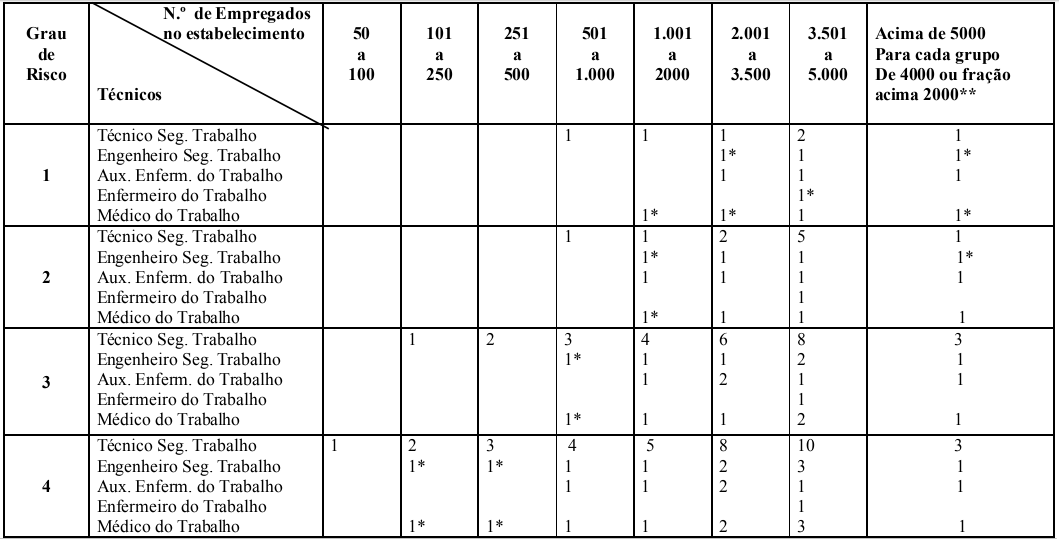
\includegraphics[scale=0.4]{quadroII_SESMT}  
  \caption{Quadro II - Anexo NR-4}  
  \label{fig:board-II_NR-4}
 \end{figure}
 
 Verificou-se o atendimento à essa NR, considerando que a empresa possui em seu quadro composição do SESMT um Engenheiro de Segurança do Trabalho e três Técnicos de Segurança do Trabalho, todos com formação e registro profissional em conformidade com o disposto na regulamentação da profissão e nos instrumentos normativos emitidos pelo respectivo Conselho Profissional. % CREA - Engenheiro de Seg, MTE - Técnicos
 
 À respeito das competências dos Serviços Especializados em Engenharia de Segurança e em Medicina do Trabalho, a empresa cumpre com todas as alíneas do item 4.12 e mantém:
 % exemplo 1
 % exemplo 2
 
 \section{NR-5 - Comissão Interna de Prevenção de Acidentes}
 A Comissão Interna de Prevenção de Acidentes - CIPA - tem como objetivo a prevenção de acidentes e doenças decorrentes do trabalho, de modo a tornar compatível permanentemente o trabalho com a preservação da vida e a promoção da saúde do trabalhador.
 
 
\end{document}

\phantompart % Finaliza a parte no bookmark do PDF para que se inicie o bookmark na raiz e adiciona espaço de parte no Sumário
%% ---
% Conclusão
% ---
\chapter{Conclusão}
% ---

% ----------------------------------------------------------
% ELEMENTOS PÓS-TEXTUAIS
% ----------------------------------------------------------
\postextual

\bibliography{abntex2-modelo-references}

%\glossary		% Consulte o manual da classe abntex2 para orientações sobre o glossário.

%% ----------------------------------------------------------
% Apêndices
% ----------------------------------------------------------
\begin{apendicesenv}
\partapendices		% Imprime uma página indicando o início dos apêndices

\chapter{Apendice A}

\end{apendicesenv}

% ----------------------------------------------------------
% Anexos
% ----------------------------------------------------------
\begin{anexosenv}
\partanexos		% Imprime uma página indicando o início dos anexos

\chapter{Anexo A}

\end{anexosenv}


%---------------------------------------------------------------------
% INDICE REMISSIVO
%---------------------------------------------------------------------
\phantompart
\printindex
%---------------------------------------------------------------------

\end{document}
